
\section{O problema do Carteiro Chinês (PCC)}

    \subsection{Grafos mistos}

    Diferentemente do problema aplicado a grafos ou digrafos, o PCC aplicado a grafos mistos não possui solução polinomial, sendo um problema NP-hard. 


    %%%%%%%%%%%%%% REF: PROBLEMA LINEAR DO KOEHLER E KAPPAUF
    %Uma solução para este caso proposta por Kappauf e Koehler\cite{mixed-pcc} que trataremos a seguir consiste em uma formulação do PCC como um problema linear inteiro.
    %%%%%%%%%%%%%%%%%%%%%%%%%%%%%%%%%%%%%%%%%%%

    %%%%%%%%%%%%%% REF: Paper do Frederickson, tem ao menos duas heuristicas pro misto ai: http://delivery.acm.org/10.1145/330000/322150/p538-frederickson.pdf?ip=195.176.178.182&id=322150&acc=ACTIVE%20SERVICE&key=FC66C24E42F07228%2E8FBBFD775A27C843%2E4D4702B0C3E38B35%2E4D4702B0C3E38B35&__acm__=1572510516_82601067be7298d3a7ff02d444c4cc9c

    Trataremos, portanto, de um algoritmo de aproximação para solucionar este problema, publicado em 1973 por Edmonds e Johnson \cite{edmonds-johnson} e posteriormente explicado em mais detalhes por Frederickson \cite{frederickson}. 

    O algoritmo é composto por três passos principais:

    \begin{enumerate}
        \item Adicionar cópias de arestas ao grafo de modo a tornar o grau de todo vértice par, considereando arcos como arestas sem orientação
        \item Igualar o grau de entrada e saída de todo vértice, adicionando cópias de arcos e orientando arestas existentes, mantendo par o grau de cada vértice
        \item Encontrar um circuito euleriano no digrafo construido
    \end{enumerate}
    

    Apresenta-se no algoritmo \ref{mixed-1} um pseudo-código adaptado de Frederickson \cite{frederickson} que segue esses passos.
    Seja $E$ o conjunto de arestas não direcionadas, $A$ o conjunto de arcos e $c$ a função de custo destas arestas e arcos.
    Tome $\delta(v)$ como a quantidade de arestas que incidem no vértice $v$, $\delta^+(v)$ como o grau de entrada de $v$, isto é, a quantidade de arcos que apontam a $v$ e $\delta^-(v)$ como o grau de saída de $v$, o número de arcos que saem de $v$.

    Definiremos como \textbf{grau total} de um vértice $v$, $\delta_t(v)$ a soma do grau de arestas não direcionadas, grau de entrada e saída, ou seja $\grt(v) = \gr(v) + \gre(v) + \grs(v)$.

    \begin{algorithm}
    \floatname{algorithm}{Algoritmo}%
    \caption{Função principal do algoritmo sugerido por Frederickson}
    \label{mixed-1}
    \begin{algorithmic}[1]
    \Function{Misto}{G, c} 
        \State $G' \gets $GRAU\_TOTAL\_PAR$(G, c)$ \Comment{Torna $\delta_t$ par}
        \State $M, U \gets $IGUALA\_GRAU\_DIR$(G', c)$ \Comment{Iguala $\delta^+$ e $\delta^-$}
        \State $M', U' \gets $GRAU\_PAR$(G', M, U)$ \Comment{Torna $\delta$ par, mantendo $\delta^+ = \delta^-$}
        \State $G_e = (V(G), U', M')$
        \State \Return CIRCUITO\_EULERIANO$(G_e)$ % TODO: Provar que tem como fazer esse circuito euleriano
    \EndFunction 
    \end{algorithmic}
    \end{algorithm}

    Para exemplificar o funcionamento do algoritmo, usaremos o seguinte grafo:

    \begin{figure}[H]
        \centering
        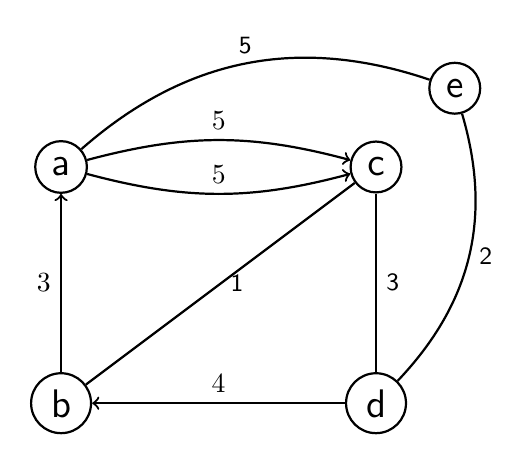
\begin{tikzpicture}[auto,node distance=3cm, every loop/.style={},thick,main node/.style={circle,draw,font=\sffamily\Large}]
            \node[main node] at (-3, 2) (a) {a};
            \node[main node] at (-3, -1) (b) {b};
            \node[main node] at (1, 2) (c) {c};
            \node[main node] at (1, -1) (d) {d};
            \node[main node] at (2, 3) (e) {e};

            \path[->] (a) edge[bend left=15] node [above] {5} (c);
            \path[->] (a) edge[bend right=15] node [above] {5} (c);
            \path[->] (b) edge[] node [left] {3} (a);
            \path[->] (d) edge[] node [above] {4} (b);

            \path[every node/.style={font=\sffamily\small}]
                (a) edge[bend left] node [above] {5} (e)
                (b) edge[] node [right] {1} (c)
                (c) edge node [right] {3} (d)
                (d) edge[bend right] node [right] {2} (e)
                ;
        \end{tikzpicture}
        \caption{Exemplo de grafo misto $G$}
        \label{mixed-exemplo}
    \end{figure}

    A função auxiliar ``GRAU\_TOTAL\_PAR'' apresentada no algoritmo \ref{mixed-grau-total-par} duplica arcos e arestas de $G$, criando um outro grafo $G'$ em que todos vértices possuem grau total par.

    Os arcos e arestas duplicados são escolhidos de modo a minimizar o custo total dos arcos e arestas de $G'$.
    
    \begin{algorithm}
    \floatname{algorithm}{Algoritmo}%
    \caption{Função auxiliar GRAU TOTAL PAR}
    \label{mixed-grau-total-par}
    \begin{algorithmic}[1]
    \Function{grau\_total\_par}{G,c}
        \State $(V, E, A) \gets G$
        \State $V' \gets \{v \in V : \delta_t(v)$ é impar$\}$
        \State $custMin \gets $ FLOYD\_WARSHALL$(G, c)$ 
            \Comment{Ignora o sentido dos arcos de $A$}
        \State $K \gets (V', V' \times V', custMin)$ 
            \Comment{Grafo completo de $V'$}
        \State $M \gets $ EMPARELHAMENTO\_PERFEITO\_MINIMO$(K)$
        \State Expande cada aresta de $M$ nos arcos e arestas do grafo original que ela representa, adicionando ao multiconjunto $A'$ os arcos expandidos e ao multiconjunto $E'$ as arestas expandidas.
        \State \Return $(V, E + E', A + A')$ 
    \EndFunction
    \end{algorithmic}
    \end{algorithm}

    \begin{figure}[H]
        \centering
        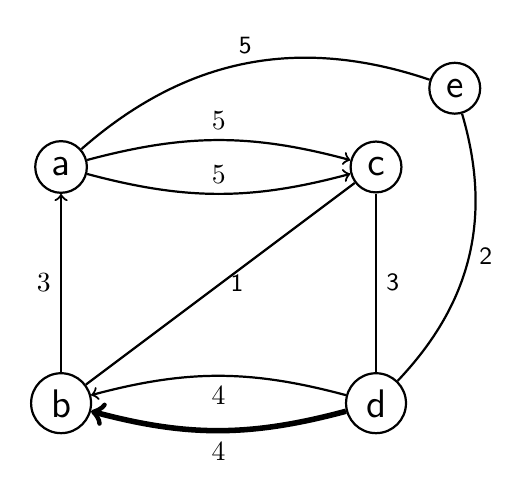
\begin{tikzpicture}[auto,node distance=3cm, every loop/.style={},thick,main node/.style={circle,draw,font=\sffamily\Large}]
            \node[main node] at (-3, 2) (a) {a};
            \node[main node] at (-3, -1) (b) {b};
            \node[main node] at (1, 2) (c) {c};
            \node[main node] at (1, -1) (d) {d};
            \node[main node] at (2, 3) (e) {e};

            \path[->] (a) edge[bend right=15] node [above] {5} (c);
            \path[->] (a) edge[bend left=15] node [above] {5} (c);
            \path[->] (b) edge[] node [left] {3} (a);
            \path[->] (d) edge[bend right=15] node [below] {4} (b);
            \path[->] (d) edge[line width=2,bend left=15] node [below] {4} (b);

            \path[every node/.style={font=\sffamily\small}]
                (a) edge[bend left] node [above] {5} (e)
                (b) edge[] node [right] {1} (c)
                (c) edge node [right] {3} (d)
                (d) edge[bend right] node [right] {2} (e)
                ;
        \end{tikzpicture}
        \caption{Em destaque o arco duplicado pela função \ref{mixed-grau-total-par}}
        \label{mixed-exemplo-grau-total}
    \end{figure}

    Por sua vez, a função ``IGUALA\_GRAU\_DIR'' devolve dois multiconjuntos $M$ e $U$, de arcos e arestas, respectivamente, de menor custo tal que todo vértice do grafo $(V, U, M)$ possui grau de entrada e saída iguais.

    O multiconjunto $M$ será formado por ao menos uma cópia de todos arcos de $A$ e cópias de arestas de $E$ direcionadas.
    Já $U$ será composto pelas arestas de $E$ que não foram direcionadas e adicionadas a $M$.

    \begin{algorithm}
    \floatname{algorithm}{Algoritmo}%
    \caption{Função auxiliar IGUALA GRAU DIR}
    \label{mixed-iguala-grau-dir}
    \begin{algorithmic}[1]
    \Function{iguala\_grau\_dir}{G, c, custMin}
    \State \Comment Devolve dois multiconjuntos $M$ e $U$, tal que $M$ contém ao menos uma cópia de cada arco de $A$ e algumas arestas de $E$ orientadas, e $U \subseteq E$ contém apenas arestas não orientadas e não pertencentes a $M$.
        \State $(V, E, A) \gets G$
        \For{$v \in V$}
            \State $b(v) \gets \delta^-(v) - \delta^+(v)$ \Comment Calcula a função demanda
        \EndFor
        \State $F \gets \{v \in V : b(v) < 0\}$
        \State $S \gets \{v \in V : b(v) > 0\}$
        \State $f \gets $ PROBLEMA\_DE\_TRANSPORTE$(F, S, custMin, b)$
        \State Seja $f_a$ a quantidade de fluxo que passa por cada arco $a \in A$ 
        \State Sejam $f_{uv}$ e $f_{vu}$ as quantidades de fluxo transportadas pelas duas orientações de uma aresta $uv \in E$

        \State $M, U \gets \emptyset$

        \For{$a \in A$}
            \State Insere $f_a + 1$ cópias do arco $a$ em $M$
        \EndFor
        \For{$uv \in E$}
            \If{$f_{vu} \geq 1$ ou $f_{uv} \geq 1$} \Comment{Se $custMin > 0$ é impossível que $f_{uv} \geq 1$ e $f_{vu} \geq 1$} ao mesmo tempo % TODO: PROVAR
                \State Insere $f_{uv}$ cópias de $uv$ e $f_{vu}$ cópias de $vu$ em $M$
            \Else 
                \State Insere $uv$ em $U$ 
            \EndIf
        \EndFor
        \State \Return $M, U$
    \EndFunction
    \end{algorithmic}
    \end{algorithm}

    \begin{figure}[H]
        \centering
        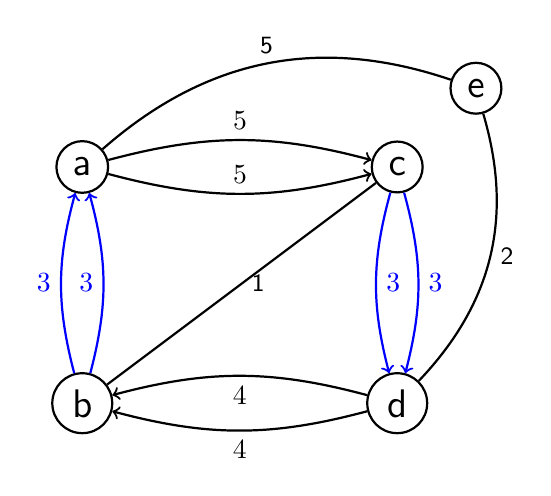
\begin{tikzpicture}[auto,node distance=3cm, every loop/.style={},thick,main node/.style={circle,draw,font=\sffamily\Large}]
            \node[main node] at (-3, 2) (a) {a};
            \node[main node] at (-3, -1) (b) {b};
            \node[main node] at (1, 2) (c) {c};
            \node[main node] at (1, -1) (d) {d};
            \node[main node] at (2, 3) (e) {e};

            \path[->] (a) edge[bend right=15] node [above] {5} (c);
            \path[->] (a) edge[bend left=15] node [above] {5} (c);
            \path[->] (b) edge[blue, bend right=15] node [left] {3} (a);
            \path[->] (b) edge[blue, bend left=15] node [left] {3} (a);
            \path[->] (d) edge[bend right=15] node [below] {4} (b);
            \path[->] (d) edge[bend left=15] node [below] {4} (b);
            \path[->] (c) edge[blue, bend right=15] node [right] {3} (d);
            \path[->] (c) edge[blue, bend left=15] node [right] {3} (d);

            \path[every node/.style={font=\sffamily\small}]
                (a) edge[bend left] node [above] {5} (e)
                (b) edge[] node [right] {1} (c)
                (d) edge[bend right] node [right] {2} (e)
                ;
        \end{tikzpicture}
        \caption{O arco $ba$ e a aresta orientada $cd$ duplicados pela função \ref{mixed-iguala-grau-dir}}
        \label{mixed-exemplo-grau-dir}
    \end{figure}

    Apesar do algoritmo \ref{mixed-iguala-grau-dir} devolver multiconjuntos $M, U$ que igualam o grau de entrada e saída dos vértices de $V$, ele não garante que grau total desses vértices continua par, como pode-se notar no exemplo da figura \ref{mixed-exemplo-grau-dir}.
    Por esse motivo é necessária a função GRAU PAR, do algoritmo \ref{mixed-grau-par}, que deriva de $M, U$ outros multiconjuntos $M'$ e $U'$ que tornam $\delta_t$ par, mantêm a igualdade de $\delta^+$ e $\delta^-$ e por consequência, tornam $\gr$ par para todo vértice.

    \begin{algorithm}
    \floatname{algorithm}{Algoritmo}%
    \caption{Função auxiliar GRAU PAR}
    \label{mixed-grau-par}
    \begin{algorithmic}[1]
        \Function{grau\_par}{G, M, U}
            %\State \Comment{Devolve os multiconjuntos $M'$, $U'$, que mantêm, para todo vértice, a igualdade dos graus $\delta^+$ e $\delta^-$ e torna $\delta^+ + \delta^- + \delta$ par.}
            \State $U' \gets U$
            \State O multiconjunto $M' \subseteq M$ deverá possuir apenas as arestas direcionadas e as cópias de arcos criadas em $GRAU\_DIR$.
            \State Seja $V' = \{v \in V : \delta^+ + \delta^- + \delta$ é ímpar $\}$

            \While{$V'$ não é vazio}
                \State Seleciona um vértice qualquer $v_{ini}$ de $V'$ 
                \State $v \gets v_{ini}$
                \While{$v \in V'$}
                    \State $V' \gets V' \setminus v$
                    \Repeat 
                        \State Seja $a$ um arco incidente a $v$, da forma $vw$ ou $wv$, pertencente a $M'$
                        \If{$a$ é o arco $vw$}
                            \State Insere outra cópia de $a$ em $M'$ \label{alg:duplica}
                        \Else
                            \State Apague uma cópia de $a$ de $M'$ \label{alg:deleta}
                        \EndIf
                        \State $v \gets w$
                    \Until{$v \notin V'$}
                    \Repeat
                        \State Remove uma aresta $vw$ de $U'$
                        \State Orienta tal aresta no sentido de $v$ para $w$ e a adiciona em $M'$ \label{alg:orienta}
                        \State $v \gets w$
                    \Until{$v \notin V'$ e $v \neq v_{ini}$}
                \EndWhile
            \EndWhile
        \EndFunction
    \end{algorithmic}
    \end{algorithm}

    \begin{figure}[H]
        \centering
        \begin{minipage}{.5\textwidth}
          \centering
            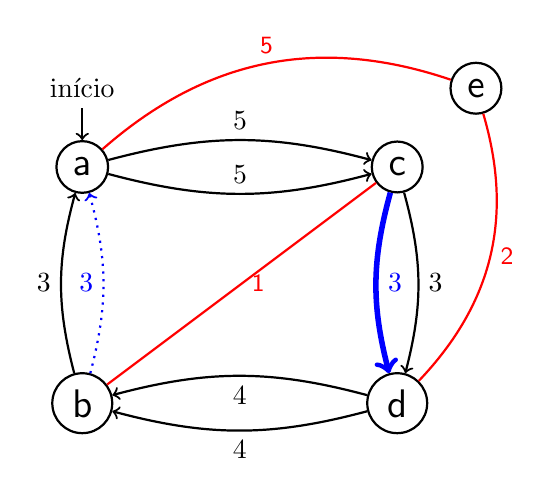
\begin{tikzpicture}[auto,node distance=3cm, every loop/.style={},thick,main node/.style={circle,draw,font=\sffamily\Large}]
                \node[main node] at (-3, 2) (a) {a};
                \node[main node] at (-3, -1) (b) {b};
                \node[main node] at (1, 2) (c) {c};
                \node[main node] at (1, -1) (d) {d};
                \node[main node] at (2, 3) (e) {e};
                \node[] at (-3, 3) (ini) {início};

                \path[->] (ini) edge[] node {} (a);

                \path[->] (a) edge[bend right=15] node [above] {5} (c);
                \path[->] (a) edge[bend left=15] node [above] {5} (c);
                \path[->] (b) edge[dotted, blue, bend right=15] node [left] {3} (a);
                \path[->] (b) edge[bend left=15] node [left] {3} (a);
                \path[->] (d) edge[bend right=15] node [below] {4} (b);
                \path[->] (d) edge[bend left=15] node [below] {4} (b);
                \path[->] (c) edge[line width=2, blue, bend right=15] node [right] {3} (d);
                \path[->] (c) edge[bend left=15] node [right] {3} (d);

                \path[every node/.style={font=\sffamily\small}]
                    (a) edge[red, bend left] node [above] {5} (e)
                    (b) edge[red] node [right] {1} (c)
                    (d) edge[red, bend right] node [right] {2} (e)
                    ;
            \end{tikzpicture}
          \label{exmixed1}
        \end{minipage}%
        \begin{minipage}{.5\textwidth}
          \centering
            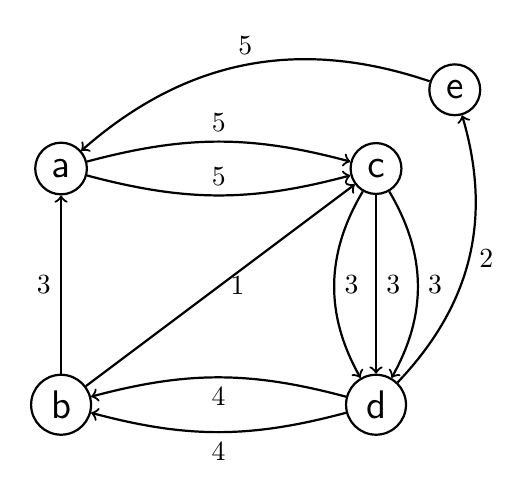
\begin{tikzpicture}[auto,node distance=3cm, every loop/.style={},thick,main node/.style={circle,draw,font=\sffamily\Large}]
                \node[main node] at (-3, 2) (a) {a};
                \node[main node] at (-3, -1) (b) {b};
                \node[main node] at (1, 2) (c) {c};
                \node[main node] at (1, -1) (d) {d};
                \node[main node] at (2, 3) (e) {e};

                \path[->] (a) edge[bend right=15] node [above] {5} (c);
                \path[->] (a) edge[bend left=15] node [above] {5} (c);
                \path[->] (b) edge[] node [left] {3} (a);
                \path[->] (d) edge[bend right=15] node [below] {4} (b);
                \path[->] (d) edge[bend left=15] node [below] {4} (b);
                \path[->] (c) edge[bend right] node [right] {3} (d);
                \path[->] (c) edge[] node [right] {3} (d);
                \path[->] (c) edge[bend left] node [right] {3} (d);
                \path[->] (b) edge[] node [right] {1} (c);
                \path[->] (d) edge[bend right] node [right] {2} (e);
                \path[->] (e) edge[bend right] node [above] {5} (a);
            \end{tikzpicture}
          \label{exmixed2}
        \end{minipage}%
        \caption{Criação de $M', U'$, a partir de $M, U$ pelo algoritmo \ref{mixed-grau-par}}
        \label{ex-grau-par}
    \end{figure}

    No exemplo \ref{ex-grau-par} o algoritmo \ref{mixed-grau-par} toma o circuito $\{a, b, c, d, e, a\}$ para realizar a construção de $M', U'$. 
    Em azul destacam-se os arcos de $M$ e em vermelho as arestas de $U$ escolhidos.

    Como o arco $ab$ é percorrido pelo circuito no sentido contrário, o mesmo é deletado do conjunto $M'$ (linha \ref{alg:deleta}), já o arco $cd$, percorrido no sentido correto, é duplicado (linha \ref{alg:duplica}).
    As arestas do circuito são todas orientadas no sentido em que são percorridas: $bc, de, ea$ (linha \ref{alg:orienta}).

    Deste modo conseguem-se multiconjuntos $M', U'$ de mesmo custo que $M, U$ e que mantêm $\gre = \grs$ e $\gr$ par para todo vértice de $G$.

    \begin{theorem} 
        Um grafo misto fortemente conexo que possui $\delta(v)$ par e $\delta^+(v) = \delta^-(v)$ para todo vértice $v$, possui um circuito euleriano.
        \label{mixed-eulerian}
    \end{theorem}

    \begin{proof}
        Seja $G = (V, E, A)$, sendo $E$ um multiconjunto de arestas e $A$ um multiconjunto de arcos.
        Definimos como $G_e$ o grafo induzido pelas arestas de $E$, e de $G_a$ o grafo induzido por $A$.
        Apesar de não necessariamente conexos, ainda valerá que todo vértice de $G_e$ possui um $\delta$ par e que todo vértice de $G_a$ tem $\gre = \grs$.
        
        $G_e$ será composto por diferentes componentes conexas com vértices de grau par, consequentemente cada componente será euleriana, pelo teorema \ref{euler}. 
        Sejam $C_1, C_2, \dots, C_k$  os circuitos eulerianos das $k$ componentes de $G_e$.

        A mesma análise pode ser feita com o grafo $G_a$, cada uma de suas componentes fortemente conexas possuirá grau de entrada e saída iguais, sendo assim grafos eulerianos pelo teorema \ref{euler-digraph}.
        Sejam $C'_1, \dots, C'_l$ os circuitos eulerianos dessas componenetes.

        Pode-se definir um procedimento de união de dois circuitos em um único circuito se ambos possuem ao menos um vértice em comum:
        
        Digamos que dois circuitos $\mathcal{C}_i$ e $\mathcal{C}_j$ possuem um vértice $v$ em comum.
        Podemos descrever ambos circuitos por seus arcos ou arestas do seguinte modo:

        \[
            \mathcal{C}_i = \{ vw_1, w_1w_2, \dots, w_nv \}
        \]
        \[
            \mathcal{C}_j = \{ vu_1, u_1u_2, \dots, u_mv \}
        \]

        Se representados desse modo, a união dos circuitos será equivalente à justaposição de ambos:

        \[
            \mathcal{C}_i \cup \mathcal{C}_j = \{ vw_1, w_1w_2, \dots w_nv, vu_1, u_1u_2, \dots, u_mv \}
        \]
        
        A união de todos circuitos $C_1, \dots C_k$ e $C'_1, \dots, C'_l$ forma um circuito euleriano do grafo original $G$.

        Como o grafo original é fortemente conexo, sempre é possível realizar a união de todos circuitos.
    Do contrário, se não houver meio de realizar tal união deverá existir um circuito $C_i$ que não possui vértice em comum com nenhum outro circuito, implicando assim que $\bigcup \mathcal{C}_i = G$ não seria fortemente conexo, contradizendo a base do raciocínio.
    \end{proof}

    Como o exemplo apresentado é transformado em um digrafo euleriano após a execução de \ref{mixed-grau-par}, basta tomar o circuito euleriano do mesmo para derivar uma solução do grafo misto original, como mostrado na figura \ref{fig:mixed-ex-sol}.


    \begin{figure}
        \begin{minipage}{.5\textwidth}
          \centering
            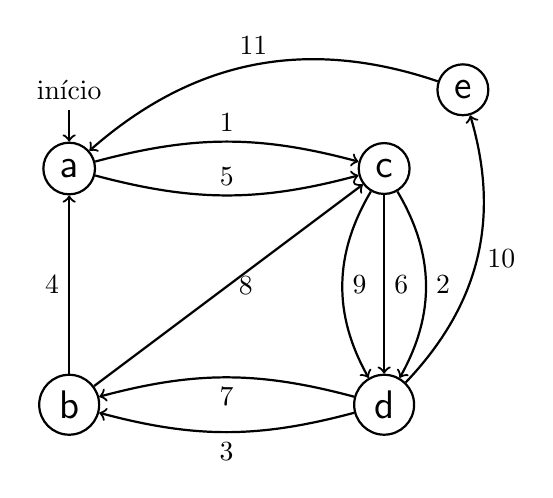
\begin{tikzpicture}[auto,node distance=3cm, every loop/.style={},thick,main node/.style={circle,draw,font=\sffamily\Large}]
                \node[main node] at (-3, 2) (a) {a};
                \node[main node] at (-3, -1) (b) {b};
                \node[main node] at (1, 2) (c) {c};
                \node[main node] at (1, -1) (d) {d};
                \node[main node] at (2, 3) (e) {e};
                \node[] at (-3, 3) (ini) {início};
                \path[->] (ini) edge[] node [] {} (a);

                \path[->] (a) edge[bend right=15] node [above] {5} (c);
                \path[->] (a) edge[bend left=15] node [above] {1} (c);
                \path[->] (b) edge[] node [left] {4} (a);
                \path[->] (d) edge[bend right=15] node [below] {7} (b);
                \path[->] (d) edge[bend left=15] node [below] {3} (b);
                \path[->] (c) edge[bend right] node [right] {9} (d);
                \path[->] (c) edge[] node [right] {6} (d);
                \path[->] (c) edge[bend left] node [right] {2} (d);
                \path[->] (b) edge[] node [right] {8} (c);
                \path[->] (d) edge[bend right] node [right] {10} (e);
                \path[->] (e) edge[bend right] node [above] {11} (a);
            \end{tikzpicture}
        \end{minipage}%
        \begin{minipage}{.5\textwidth}
            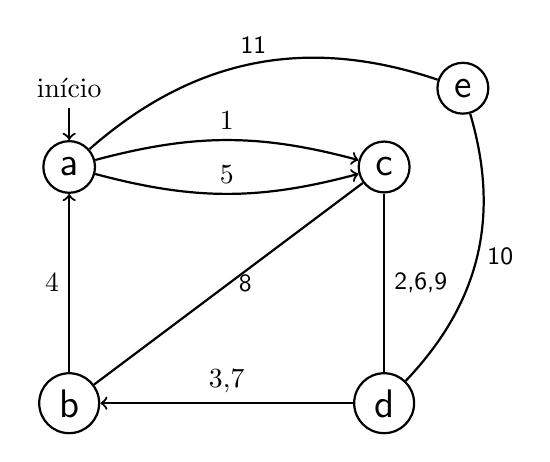
\begin{tikzpicture}[auto,node distance=3cm, every loop/.style={},thick,main node/.style={circle,draw,font=\sffamily\Large}]
                \node[main node] at (-3, 2) (a) {a};
                \node[main node] at (-3, -1) (b) {b};
                \node[main node] at (1, 2) (c) {c};
                \node[main node] at (1, -1) (d) {d};
                \node[main node] at (2, 3) (e) {e};
                \node[] at (-3, 3) (ini) {início};
                \path[->] (ini) edge[] node [] {} (a);

                \path[->] (a) edge[bend left=15] node [above] {1} (c);
                \path[->] (a) edge[bend right=15] node [above] {5} (c);
                \path[->] (b) edge[] node [left] {4} (a);
                \path[->] (d) edge[] node [above] {3,7} (b);

                \path[every node/.style={font=\sffamily\small}]
                    (a) edge[bend left] node [above] {11} (e)
                    (b) edge[] node [right] {8} (c)
                    (c) edge node [right] {2,6,9} (d)
                    (d) edge[bend right] node [right] {10} (e)
                    ;
            \end{tikzpicture}
        \end{minipage}
        \caption{Circuito euleriano de $G_e$ e solução do PCC de $G$, respectivamente}
        \label{fig:mixed-ex-sol}
    \end{figure}

    \begin{lemma}
        \label{mixed-custo-igual}
        Seja $C(M,U)$ o custo dos multiconjuntos $M,U$, ou seja, a soma do custo dos arcos e arestas que compõem $M$ e $U$.

        Vale que $C(M', U') = C(M, U)$. 
        Isto é, os multiconjuntos $M', U'$ retornados pela função \ref{mixed-grau-par} possuem o mesmo custo que os multiconjuntos $M, U$, retornados por \ref{mixed-iguala-grau-dir}.
    \end{lemma}

    \begin{proof}
        Como os conjuntos $M, U$ foram gerados resolvendo um problema de transporte, possuimos a garantia que eles são os multiconjuntos de menor custo que igualam o grau de entrada e saída de todos vértices de um grafo $G(V, A, E)$. 
        Em particular, vale que $C(M', U') \geq C(M, U)$. 

        Para mostrar que $C(M', U') = C(M, U)$ chegaremos a uma contradição assumindo que $C(M', U') > C(M, U)$:

        Os multiconjuntos $M'$ e $U'$ são construidos pelo algoritmo \ref{mixed-grau-par} a partir de $M$ e $U$. 
        Como exemplificado na figura \ref{ex-grau-par} na construção de $M', U'$ podem ocorrer três tipos de eventos:

        \begin{enumerate}
            \item Um arco $a \in M$ é duplicado em $M'$
            \item Um arco $a \in M$ é deletado em $M'$
            \item Uma aresta $e \in U$ é orientada e adicionada a $M'$
        \end{enumerate}
        
        Dos três tipos de eventos listados, apenas os dois primeiros mudam o custo dos multiconjuntos $M', U'$ em relação a $M, U$.
        Um evento do tipo 1 aumenta o custo de $M', U'$ pelo valor do custo de $a$, assim como um evento do tipo 2 diminui o custo de $M', U'$ pelo custo de $a$, em relação ao custo de $M, U$.

        Sendo assim, podemos definir $C(M', U')$ como $C(M', U') = C(M, U) + C_+ - C_-$, sendo $C_+$ a soma do custo dos arcos duplicados (evento 1) e $C_-$ a soma do custo dos arcos deletados no algoritmo (evento 2).

        Se $C(M', U') > C(M, U)$, como assumimos, vale que:

        \begin{align*}
            C(M, U) + C_+ - C_- &= C(M', U') \\
            C_+ - C_- &= C(M', U') - C(M, U) \\
            C_+ - C_- &> 0 \\ 
        \end{align*}

        Vamos tomar agora outros multiconjuntos $M'', U''$, em que $U'' = U'$ e que $M''$ será definido a partir de $M$ com três eventos, de modo análogo a $M'$:
        
        \begin{enumerate}
            \item Se um arco $a \in M$ foi duplicado em $M'$, o mesmo será deletado de $M''$.
            \item Se um arco $a \in M$ foi deletado em $M'$, o mesmo será duplicado em $M''$.
            \item Se uma aresta $e \in U$ foi orientada da forma $uv$ e adicionada a $M'$, a mesma será adicionada a $M''$ com a orientação oposta: $vu$.
        \end{enumerate}

        Para exemplificar essa definição, na figura \ref{fig:mixed-ex-lema} comparam-se os conjuntos $M', U'$ e $M'', U''$ do exemplo tratado nesta seção.

        \begin{figure}[H]
            \centering
            \begin{minipage}{.5\textwidth}
              \centering
                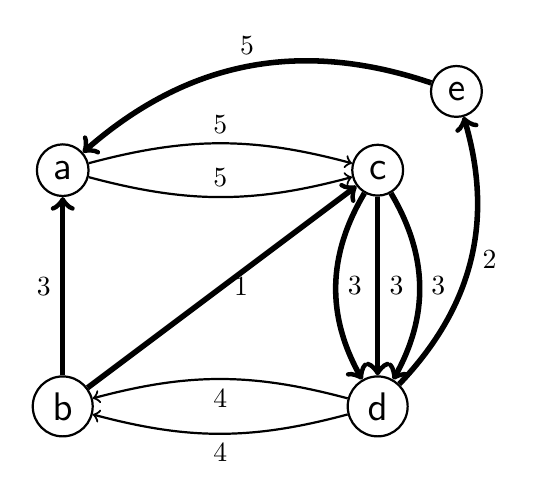
\begin{tikzpicture}[auto,node distance=3cm, every loop/.style={},thick,main node/.style={circle,draw,font=\sffamily\Large}]
                    \node[main node] at (-3, 2) (a) {a};
                    \node[main node] at (-3, -1) (b) {b};
                    \node[main node] at (1, 2) (c) {c};
                    \node[main node] at (1, -1) (d) {d};
                    \node[main node] at (2, 3) (e) {e};

                    \path[->] (a) edge[bend right=15] node [above] {5} (c);
                    \path[->] (a) edge[bend left=15] node [above] {5} (c);
                    \path[->] (b) edge[line width=2] node [left] {3} (a);
                    \path[->] (d) edge[bend right=15] node [below] {4} (b);
                    \path[->] (d) edge[bend left=15] node [below] {4} (b);
                    \path[->] (c) edge[line width=2, bend right] node [right] {3} (d);
                    \path[->] (c) edge[line width=2] node [right] {3} (d);
                    \path[->] (c) edge[line width=2, bend left] node [right] {3} (d);
                    \path[->] (b) edge[line width=2] node [right] {1} (c);
                    \path[->] (d) edge[line width=2, bend right] node [right] {2} (e);
                    \path[->] (e) edge[line width=2, bend right] node [above] {5} (a);
                \end{tikzpicture}
            \end{minipage}%
            \begin{minipage}{.5\textwidth}
              \centering
                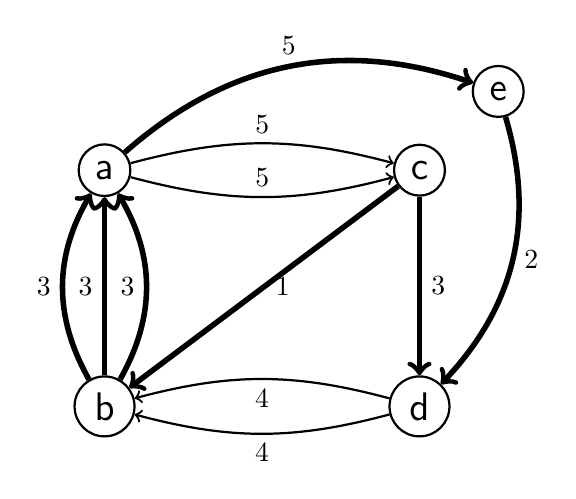
\begin{tikzpicture}[auto,node distance=3cm, every loop/.style={},thick,main node/.style={circle,draw,font=\sffamily\Large}]
                    \node[main node] at (-3, 2) (a) {a};
                    \node[main node] at (-3, -1) (b) {b};
                    \node[main node] at (1, 2) (c) {c};
                    \node[main node] at (1, -1) (d) {d};
                    \node[main node] at (2, 3) (e) {e};

                    \path[->] (a) edge[bend right=15] node [above] {5} (c);
                    \path[->] (a) edge[bend left=15] node [above] {5} (c);
                    \path[->] (b) edge[line width=2, bend right] node [left] {3} (a);
                    \path[->] (b) edge[line width=2, bend left] node [left] {3} (a);
                    \path[->] (b) edge[line width=2] node [left] {3} (a);
                    \path[->] (d) edge[bend right=15] node [below] {4} (b);
                    \path[->] (d) edge[bend left=15] node [below] {4} (b);
                    \path[->] (c) edge[line width=2] node [right] {3} (d);
                    \path[->] (c) edge[line width=2] node [right] {1} (b);
                    \path[->] (e) edge[line width=2, bend left] node [right] {2} (d);
                    \path[->] (a) edge[line width=2, bend left] node [above] {5} (e);
                \end{tikzpicture}
            \end{minipage}%
            \caption{ Diferenças entre $M', U'$ e $M'', U''$, respectivamente}
            \label{fig:mixed-ex-lema}
        \end{figure}

        Como $M'', U''$ também igualam os graus de entrada e saída de $G$, então vale que $C(M'', U'') \geq C(M, U)$.
        Além disso, podemos definir tal custo como $C(M'', U'') = C(M, U) + C_- - C_+$.
        
        Sendo assim:

        \begin{align*}
            C(M, U) + C_- - C_+ &= C(M'', U'') \\
            C_+ - C_- &= C(M, U) - C(M'', U'') \\
            C_+ - C_- &\leq 0 
        \end{align*}

        Como haviamos provado anteriormente que $C_+ - C_- > 0$, chegamos a uma contradição.
        Provando por absurdo, que $C(M', U') = C(M, U)$.
    \end{proof}

    \begin{theorem}{\cite{frederickson}}
        Seja $C$ o custo de uma solução ótima do problema do carteiro chinês em um grafo misto $G$, e $C'$ o custo da solução construída pelo algoritmo descrito, vale que:
        \[
            C'/C \leq 2
        \]
    \end{theorem}

    \begin{proof}
        Assume-se que todas arestas e arcos de $G$ tenham um custo positivo. 

        Seja $G^*$ o grafo $G$ com todos arcos e arestas duplicadas e $C^*$ o custo da solução dada pelo algoritmo MISTO ao grafo $G^*$.

        Como o grau total de todos vértices de $G^*$ é par, as únicas funções que modificarão o grafo $G^*$ do algoritmo serão \ref{mixed-iguala-grau-dir} e \ref{mixed-grau-par}.
        Além disso, como a função \ref{mixed-iguala-grau-dir} encontra multiconjuntos de arcos e arestas que igualam os graus de entrada e saída de $G^*$ com o menor custo possível (solucionando o problema de transporte modelado) e como a função \ref{mixed-grau-par} modifica os multiconjuntos sem modificar o seu custo (lema \ref{mixed-custo-igual}), podemos dizer que $C^*$ é o custo ótimo para a solução do PCC para o grafo misto $G^*$. 

        Sendo assim, como a solução ótima de $G$, de custo $C$, pode ser duplicada para encontrar uma solução de $G^*$ também deve valer que $C^* \leq 2C$.

        Definimos agora $G'$ como o grafo retornado pela função \ref{mixed-grau-total-par} com parâmetro $G$.
        A função \ref{mixed-grau-total-par} constrói $G'$ duplicando arcos e arestas de caminhos entre vértices de grau total ímpar de $G$, minimizando o custo de tal construção.

        Pode-se afirmar que não existirá em $G'$ um arco ou aresta $uv$ que foi duplicado mais que uma vez na função \ref{mixed-grau-total-par}, pois se existisse poderia-se remover de $G'$ duas cópias de $uv$ que conseguiria-se outro grafo com mesma paridade total de vértices e custo menor.

        Assim, como cada aresta e arco de $G$ é duplicado no máximo uma vez em $G'$, podemos afirmar que os multiconjuntos de arcos e arestas de $G'$ estarão contidos nos multiconjuntos de $G^*$ e por isso, o custo $C'$ da solução dada pelo algoritmo MISTO ao grafo $G$ deverá ser menor ou igual a $C^*$.
        
        \begin{align*}
            C' \leq C^* &\leq 2C \\
            C'/C &\leq 2
        \end{align*}

        Provando assim que o algoritmo MISTO é uma 0.5-aproximação para o problema do carteiro misto.
    \end{proof}

